% DepthLSSTransform / LSSTransform detail (BEVFusion camera view transform).
\documentclass[tikz,border=8pt]{standalone}
% Shared styles for the DSB architecture diagrams.
\usepackage[T1]{fontenc}
\usepackage{graphicx}
\usetikzlibrary{arrows.meta, backgrounds, calc, fit, positioning, shapes.geometric}

\definecolor{camA}{HTML}{2A78D6}
\definecolor{lidA}{HTML}{1BAF7A}
\definecolor{fusA}{HTML}{EB6834}
\definecolor{detA}{HTML}{6250D6}
\definecolor{segA}{HTML}{0E8FA8}
\definecolor{occA}{HTML}{B5482A}
\definecolor{inkA}{HTML}{262626}
\definecolor{mutA}{HTML}{6B6B6B}

\tikzset{
  blk/.style={
    draw=inkA!70, line width=0.45pt, rounded corners=2.5pt,
    align=center, font=\small, inner sep=3pt,
    minimum height=0.95cm, text=inkA, fill=white,
  },
  cam/.style={blk, fill=camA!10, draw=camA!75},
  lid/.style={blk, fill=lidA!10, draw=lidA!75},
  fus/.style={blk, fill=fusA!12, draw=fusA!80},
  det/.style={blk, fill=detA!10, draw=detA!75},
  seg/.style={blk, fill=segA!10, draw=segA!75},
  occ/.style={blk, fill=occA!10, draw=occA!75},
  io/.style={blk, fill=black!4, draw=inkA!55},
  arr/.style={-{Stealth[length=2.2mm,width=1.6mm]}, line width=0.65pt, draw=inkA!75},
  darr/.style={arr, dashed},
  tag/.style={font=\scriptsize, text=mutA},
  grp/.style={draw=mutA!70, dashed, line width=0.6pt, rounded corners=6pt, inner sep=8pt},
  hdr/.style={font=\normalsize\bfseries, text=inkA, anchor=west},
  note/.style={font=\scriptsize, text=mutA, align=left},
}


\begin{document}
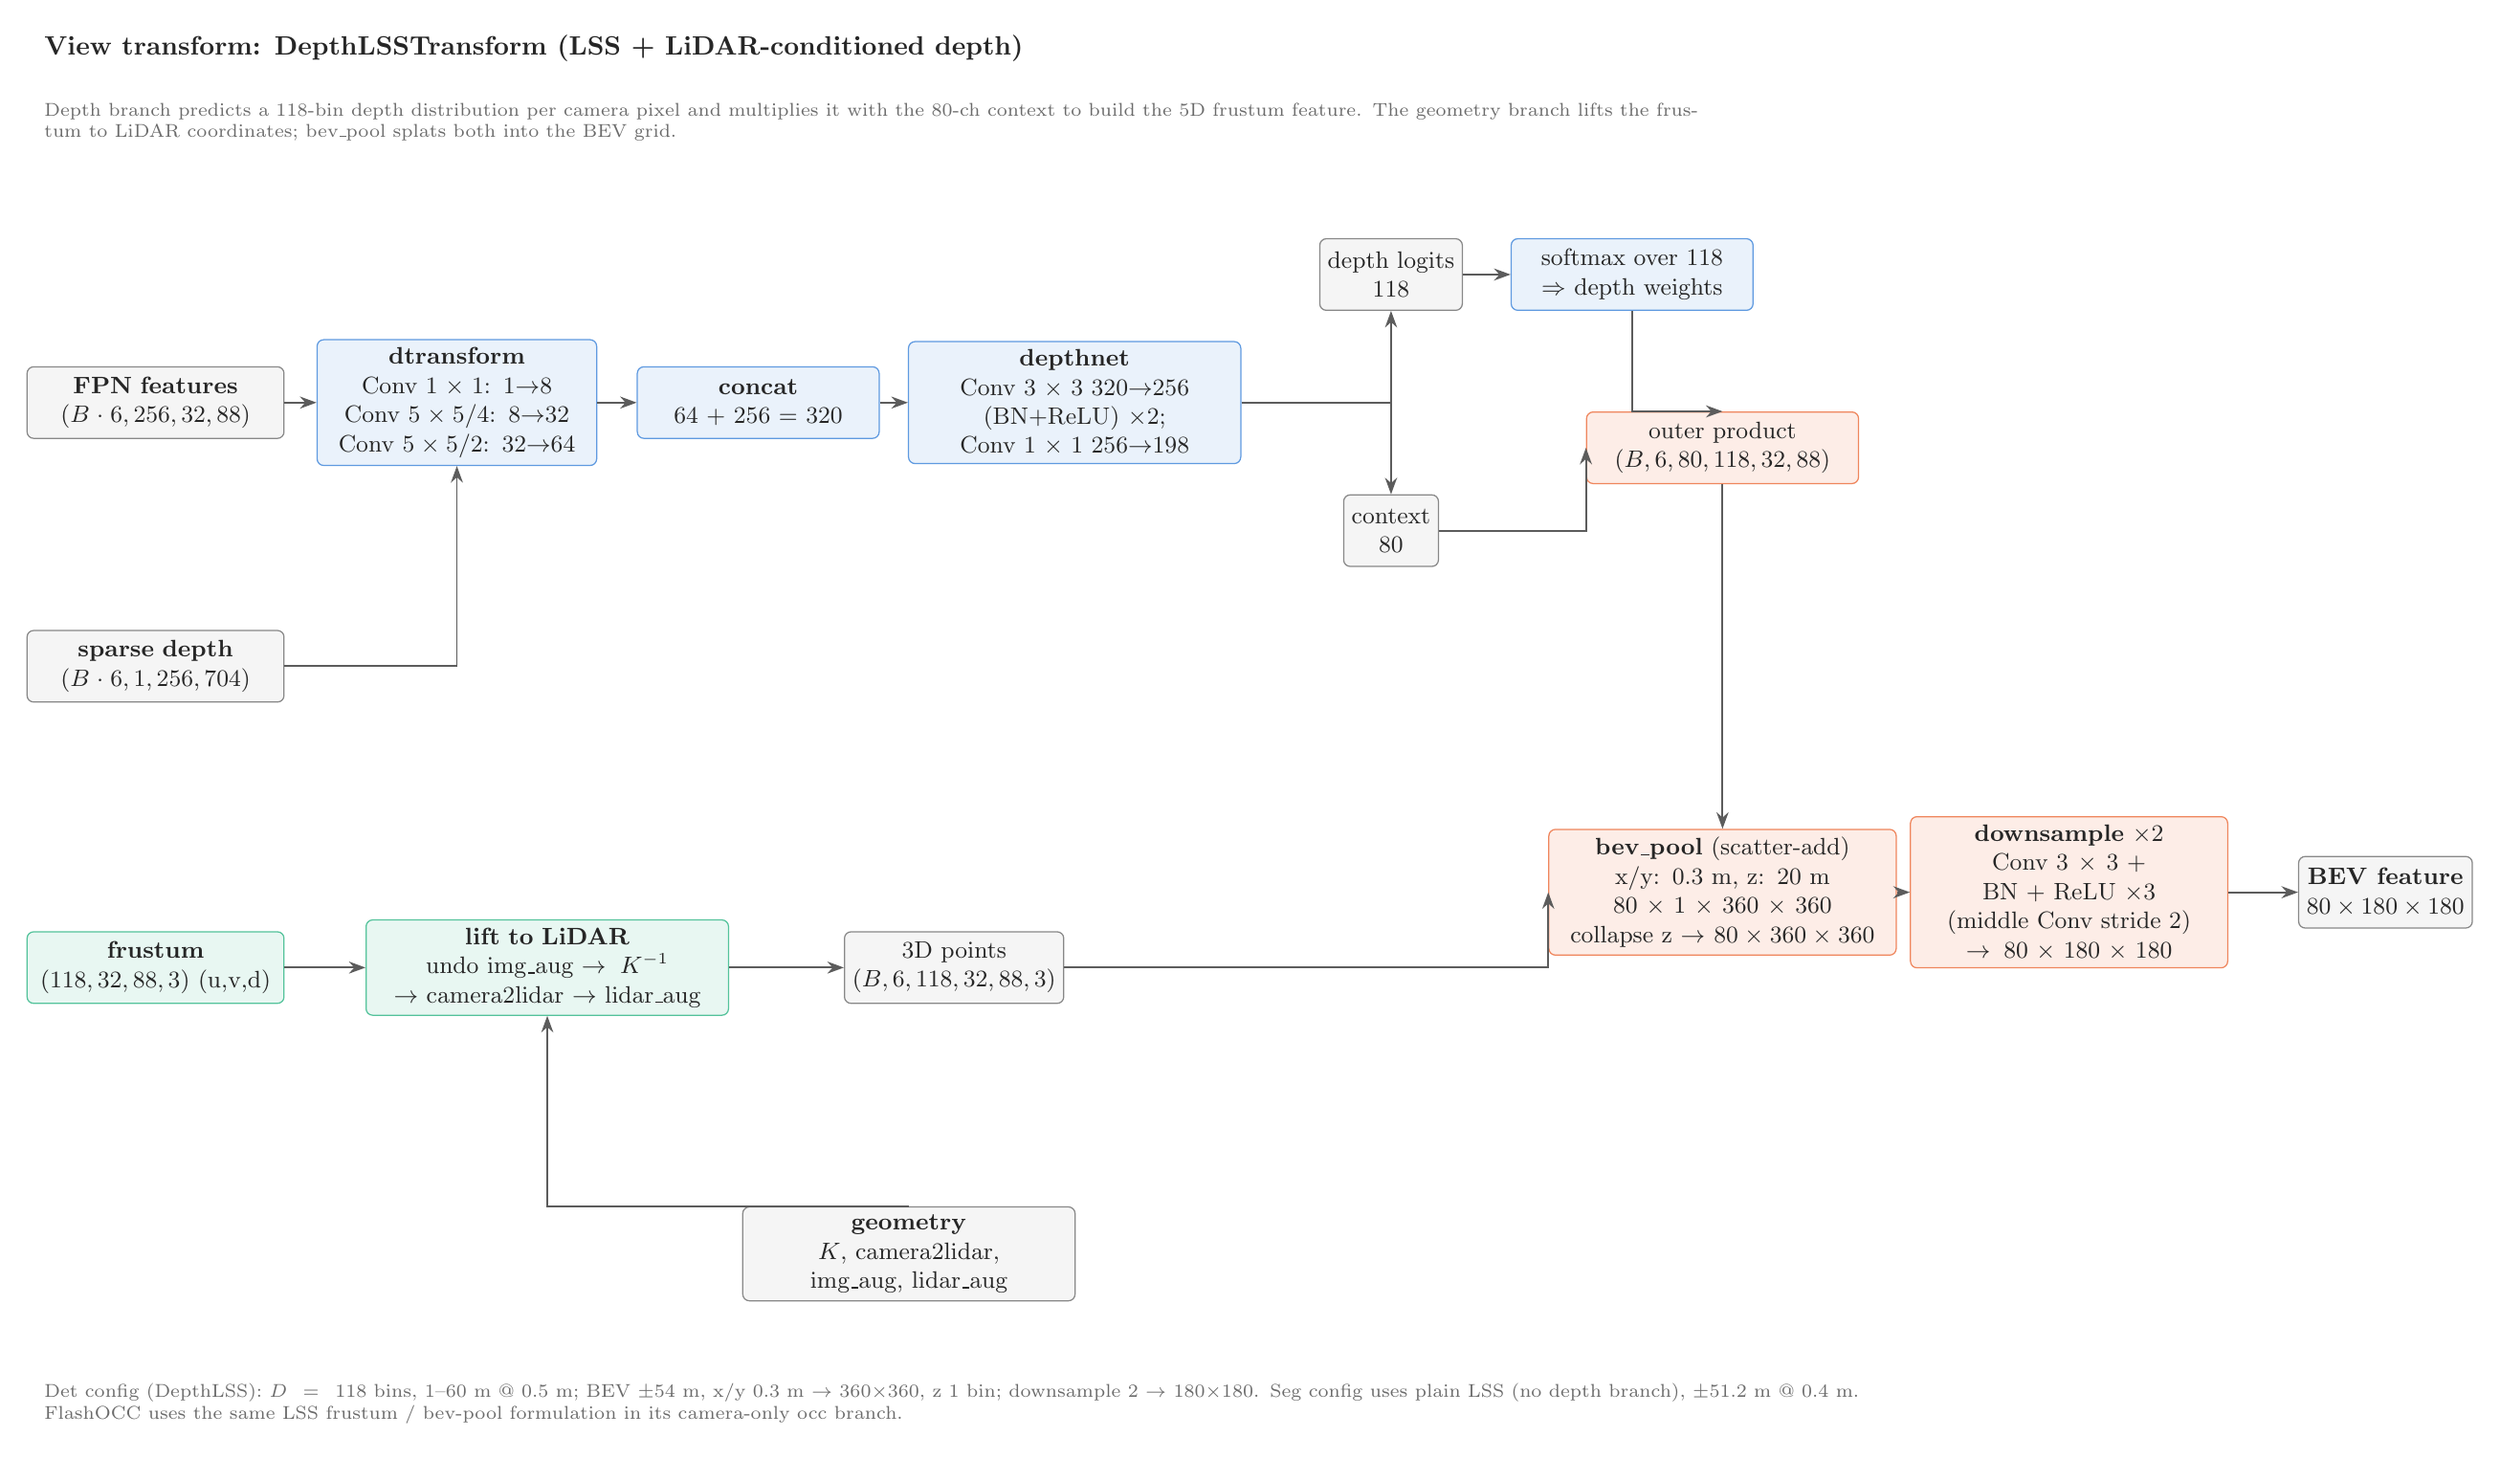
\begin{tikzpicture}

% ---------------------------------------------------------------- inputs
\node[io, text width=3.2cm] (feat) at (0,13.5)
  {\textbf{FPN features}\\$(B\cdot6,256,32,88)$};
\node[io, text width=3.2cm] (depth) at (0,10.0)
  {\textbf{sparse depth}\\$(B\cdot6,1,256,704)$};
\node[io, text width=4.2cm] (mats) at (10.0,2.2)
  {\textbf{geometry}\\$K$, camera2lidar, img\_aug, lidar\_aug};

% ---------------------------------------------------------------- depth/context
\node[cam, text width=3.5cm] (dtr) at (4.0,13.5)
  {\textbf{dtransform}\\Conv $1\times1$: 1$\to$8\\
   Conv $5\times5$/4: 8$\to$32\\Conv $5\times5$/2: 32$\to$64};
\node[cam, text width=3.0cm] (cat) at (8.0,13.5)
  {\textbf{concat}\\64 + 256 = 320};
\node[cam, text width=4.2cm] (dnet) at (12.2,13.5)
  {\textbf{depthnet}\\Conv $3\times3$ 320$\to$256\\
   (BN+ReLU) $\times2$; Conv $1\times1$ 256$\to$198};

\node[io] (dlog) at (16.4,15.2) {depth logits\\118};
\node[io] (ctx)  at (16.4,11.8) {context\\80};
\node[cam, text width=3.0cm] (soft) at (19.6,15.2)
  {softmax over 118\\$\Rightarrow$ depth weights};
\node[fus, text width=3.4cm] (outer) at (20.8,12.9)
  {outer product\\$(B,6,80,118,32,88)$};

\draw[arr] (feat) -- (dtr);
\draw[arr] (depth.east) -| (dtr.south);
\draw[arr] (dtr) -- (cat);
\draw[arr] (cat) -- (dnet);
\draw[arr] (dnet.east) -| (dlog.south);
\draw[arr] (dnet.east) -| (ctx.north);
\draw[arr] (dlog) -- (soft);
\draw[arr] (soft.south) |- (outer.north);
\draw[arr] (ctx.east) -| (outer.west);

% ---------------------------------------------------------------- geometry
\node[lid, text width=3.2cm] (frus) at (0,6.0)
  {\textbf{frustum}\\$(118,32,88,3)$ (u,v,d)};
\node[lid, text width=4.6cm] (geom) at (5.2,6.0)
  {\textbf{lift to LiDAR}\\undo img\_aug $\to K^{-1}$\\
   $\to$ camera2lidar $\to$ lidar\_aug};
\node[io] (pts) at (10.6,6.0) {3D points\\$(B,6,118,32,88,3)$};
\draw[arr] (frus) -- (geom);
\draw[arr] (geom) -- (pts);
\draw[arr] (mats.north) -| (geom.south);

% ---------------------------------------------------------------- bev pool + downsample
\node[fus, text width=4.4cm] (pool) at (20.8,7.0)
  {\textbf{bev\_pool} (scatter-add)\\x/y: 0.3 m, z: 20 m\\
   $80\times1\times360\times360$\\collapse z $\to 80\times360\times360$};
\node[fus, text width=4.0cm] (down) at (25.4,7.0)
  {\textbf{downsample} $\times2$\\Conv $3\times3$ + BN + ReLU $\times3$\\
   (middle Conv stride 2)\\$\to 80\times180\times180$};
\node[io] (out) at (29.6,7.0) {\textbf{BEV feature}\\$80\times180\times180$};

\draw[arr] (outer.south) -- (pool.north);
\draw[arr] (pts.east) -| (pool.west);
\draw[arr] (pool) -- (down);
\draw[arr] (down) -- (out);

% ---------------------------------------------------------------- notes
\node[note, anchor=north west, text width=25cm] at (-1.6,0.6)
  {Det config (DepthLSS): $D=118$ bins, 1--60 m @ 0.5 m; BEV $\pm$54 m, x/y 0.3 m $\to$ 360$\times$360, z 1 bin;
    downsample 2 $\to$ 180$\times$180. Seg config uses plain LSS (no depth branch), $\pm$51.2 m @ 0.4 m.
    FlashOCC uses the same LSS frustum / bev-pool formulation in its camera-only occ branch.};

\node[hdr] at (-1.6,18.2) {View transform: DepthLSSTransform (LSS + LiDAR-conditioned depth)};
\node[note, anchor=north west, text width=22cm] at (-1.6,17.6)
  {Depth branch predicts a 118-bin depth distribution per camera pixel and multiplies it with the 80-ch context
   to build the 5D frustum feature. The geometry branch lifts the frustum to LiDAR coordinates; bev\_pool splats
   both into the BEV grid.};

\end{tikzpicture}
\end{document}
